\titledquestion{Alphabet Cognitive Battle}

Consider the AVL tree below. Each symbol represents a unique object stored in the AVL tree.


\begin{tikzpicture}[]
\Tree
[.$\alpha$
    [.$\beta$
        [.$\delta$
        ]
        [.$\phi$
        ]
    ]
    [.$\gamma$
        \edge[blank]; \node[blank]{};
        [.$\kappa$
        ]
    ]
]
\end{tikzpicture}

The following 4 questions are \textbf{independent} of each other, i.e. for each question, your answer should be built on the original AVL Tree above, instead of the AVL Tree from the answer of the last question.

\begin{parts}

\part[3] If we delete object $\gamma$, then insert object $\gamma$, then insert new object $\epsilon$ ($\gamma < \epsilon < \kappa$), please draw the AVL tree after each insert/delete operation.

\begin{solution}
    \begin{center}
        \begin{tikzpicture}[]
            \Tree
            [.$\alpha$
                [.$\beta$
                    [.$\delta$
                    ]
                    [.$\phi$
                    ]
                ]
                [.$\kappa$
                ]
            ]
        \end{tikzpicture}
        \\
        \vspace{2cm}
        \begin{tikzpicture}[]
            \Tree
            [.$\alpha$
                [.$\beta$
                    [.$\delta$
                    ]
                    [.$\phi$
                    ]
                ]
                [.$\kappa$
                    [.$\gamma$
                    ]
                    \edge[blank]; \node[blank]{};
                ]
            ]
        \end{tikzpicture}
        \\
        \vspace{2cm}
        \begin{tikzpicture}[]
            \Tree
            [.$\alpha$
                [.$\beta$
                    [.$\delta$
                    ]
                    [.$\phi$
                    ]
                ]
                [.$\gamma$
                    [.$\epsilon$
                    ]
                    [.$\kappa$
                    ]
                ]
            ]
        \end{tikzpicture}
    \end{center}
\end{solution}


\part[3] If we want to insert a new object $\epsilon$ (not equal to the 6 objects)but we don’t want to change the tree’s current structure to maintain balance. What are the ranges of the object we can insert? (Note: the range is denoted by the objects, for example, $\alpha < \epsilon < \beta, \epsilon < \delta)$.

\begin{solution}

$ \epsilon < \gamma$ 

\end{solution}

\part[2] If we know the last object we insert is $\phi$. What is the tree before inserting it? Symbols must be unique. You may only use the 6 printed symbols. If there are more than 3 correct answers, giving only 3 correct answers would lead to full credit.

\begin{solution}
    \begin{center}
        \begin{tikzpicture}[]
            \Tree
            [.$\alpha$
                [.$\beta$
                    [.$\delta$
                    ]
                    \edge[blank]; \node[blank]{};
                ]
                [.$\gamma$
                    \edge[blank]; \node[blank]{};
                    [.$\kappa$
                    ]
                ]
            ]
        \end{tikzpicture}
        \\
        \vspace{2cm}
    \begin{tikzpicture}[]
            \Tree
            [.$\alpha$
                [.$\delta$
                    \edge[blank]; \node[blank]{};
                    [.$\beta$ 
                    ]
                ]
                [.$\gamma$
                    \edge[blank]; \node[blank]{};
                    [.$\kappa$
                    ]
                ]
            ]
    \end{tikzpicture}
    \\
    \vspace{2cm}
    \begin{tikzpicture}[]
        \Tree
        [.$\gamma$
            [.$\beta$
                [.$\delta$ 
                ]
                [.$\alpha$
                ]
            ]
            [.$\kappa$
            ]
        ]
    \end{tikzpicture}
    \end{center}
\end{solution}


\part[3] If we don’t know the last object we insert, but we know we change the tree’s structure to maintain balance. What is the object we may insert? Please write down the possible objects. Symbols must be unique. You may only use the 6 printed symbols. If there are more than 3 correct answers, giving only 3 correct answers would lead to full credit. Giving any wrong answer will lead to zero credit.

\begin{solution}
    \begin{center}
        object $\phi$, As we have shown in the previous question\\
        \vspace{1cm}
        object $\beta$
        \begin{tikzpicture}[]
            \Tree
            [.$\alpha$
                [.$\phi$
                    [ .$\delta$
                    ]
                    \edge[blank]; \node[blank]{};
                ]
                [.$\gamma$
                    \edge[blank]; \node[blank]{};
                    [.$\kappa$
                    ]
                ]
            ]
        \end{tikzpicture}
        \\
        \vspace{1cm}
        object $\delta$
        \begin{tikzpicture}[]
            \Tree
            [.$\alpha$
                [.$\phi$
                    [.$\beta$
                    ]
                    \edge[blank]; \node[blank]{};
                ]
                [.$\gamma$
                    \edge[blank]; \node[blank]{};
                    [.$\kappa$
                    ]
                ]
            ]
        \end{tikzpicture}
    \end{center}
\end{solution}

\end{parts}